
\documentclass[letterpaper,hide notes,xcolor={table,svgnames},pdftex,10pt]{beamer}
\def\showexamples{t}

\usecolortheme{crane}
\setbeamertemplate{navigation symbols}{}

\usetheme{MyPittsburgh}
\usepackage{hyperref}
\usepackage{graphicx,xspace}
\usepackage[normalem]{ulem}
\usepackage{multicol}
\usepackage{amsmath,amssymb,amsthm,graphicx,xspace}
\newcommand\SF[1]{$\bigstar$\footnote{SF: #1}}

\usepackage[sfdefault,lf]{carlito}
\usepackage[T1]{fontenc}
\usepackage[scaled]{beramono}
\usepackage{tikzpagenodes}
\newcommand{\Rplus}{\protect\hspace{-.1em}\protect\raisebox{.35ex}{\small{\small\textbf{+}}}}
\newcommand{\Cpp}{\mbox{C\Rplus\Rplus}\xspace}

\newcounter{tmpnumSlide}
\newcounter{tmpnumNote}

\newcommand\mnote[1]{%
	\addtocounter{tmpnumSlide}{1}
	\ifdefined\showcues {~\tiny\fbox{\arabic{tmpnumSlide}}}\fi
	\note{\setlength{\parskip}{1ex}\addtocounter{tmpnumNote}{1}\textbf{\Large \arabic{tmpnumNote}:} {#1\par}}}

\newcommand\mmnote[1]{\note{\setlength{\parskip}{1ex}#1\par}}


\newcommand\mquestion[2]{{~\color{red}\fbox{?}}\note{\setlength{\parskip}{1ex}\par{\Large \textbf{?}} #1} \note{\setlength{\parskip}{1ex}\par{\Large \textbf{A}} #2\par}\ifdefined \presentationonly \pause \fi}

\newcommand\blackboard[1]{%
	\ifdefined   \showblackboard
		{#1}
	\else {\begin{center} \fbox{\colorbox{blue!30}{%
						\begin{minipage}{.95\linewidth}%
							\hspace{\stretch{1}} Some space intentionally left blank; done at the blackboard.%
						\end{minipage}}}\end{center}}%
	\fi%
}

\usepackage{listings}
\lstset{%
	keywordstyle=\bfseries,
	aboveskip=15pt,
	belowskip=15pt,
	captionpos=b,
	identifierstyle=\ttfamily,
	frame=lines,
	numbers=left, basicstyle=\scriptsize, numberstyle=\tiny, stepnumber=0, numbersep=2pt}

\usepackage{siunitx}
\newcommand\sius[1]{\num[group-separator = {,}]{#1}\si{\micro\second}}
\newcommand\sims[1]{\num[group-separator = {,}]{#1}\si{\milli\second}}
\newcommand\sins[1]{\num[group-separator = {,}]{#1}\si{\nano\second}}
\sisetup{group-separator = {,}, group-digits = true}

%% -------------------- tikz --------------------
\usepackage{tikz}
\usetikzlibrary{positioning}
\usetikzlibrary{arrows,backgrounds,automata,decorations.shapes,decorations.pathmorphing,decorations.markings,decorations.text}

\tikzstyle{place}=[circle,draw=blue!50,fill=blue!20,thick, inner sep=0pt,minimum size=6mm]
\tikzstyle{transition}=[rectangle,draw=black!50,fill=black!20,thick, inner sep=0pt,minimum size=4mm]

\tikzstyle{block}=[rectangle,draw=black, thick, inner sep=5pt]
\tikzstyle{bullet}=[circle,draw=black, fill=black, thin, inner sep=2pt]

\tikzstyle{pre}=[<-,shorten <=1pt,>=stealth',semithick]
\tikzstyle{post}=[->,shorten >=1pt,>=stealth',semithick]
\tikzstyle{bi}=[<->,shorten >=1pt,shorten <=1pt, >=stealth',semithick]

\tikzstyle{mut}=[-,>=stealth',semithick]

\tikzstyle{treereset}=[dashed,->, shorten >=1pt,>=stealth',thin]

\usepackage{ifmtarg}
\usepackage{xifthen}
\makeatletter
% new counter to now which frame it is within the sequence
\newcounter{multiframecounter}
% initialize buffer for previously used frame title
\gdef\lastframetitle{\textit{undefined}}
% new environment for a multi-frame
\newenvironment{multiframe}[1][]{%
	\ifthenelse{\isempty{#1}}{%
		% if no frame title was set via optional parameter,
		% only increase sequence counter by 1
		\addtocounter{multiframecounter}{1}%
	}{%
		% new frame title has been provided, thus
		% reset sequence counter to 1 and buffer frame title for later use
		\setcounter{multiframecounter}{1}%
		\gdef\lastframetitle{#1}%
	}%
	% start conventional frame environment and
	% automatically set frame title followed by sequence counter
	\begin{frame}%
		\frametitle{\lastframetitle~{\normalfont(\arabic{multiframecounter})}}%
		}{%
	\end{frame}%
}
\makeatother

\makeatletter
\newdimen\tu@tmpa%
\newdimen\ydiffl%
\newdimen\xdiffl%
\newcommand\ydiff[2]{%
	\coordinate (tmpnamea) at (#1);%
	\coordinate (tmpnameb) at (#2);%
	\pgfextracty{\tu@tmpa}{\pgfpointanchor{tmpnamea}{center}}%
	\pgfextracty{\ydiffl}{\pgfpointanchor{tmpnameb}{center}}%
	\advance\ydiffl by -\tu@tmpa%
}
\newcommand\xdiff[2]{%
	\coordinate (tmpnamea) at (#1);%
	\coordinate (tmpnameb) at (#2);%
	\pgfextractx{\tu@tmpa}{\pgfpointanchor{tmpnamea}{center}}%
	\pgfextractx{\xdiffl}{\pgfpointanchor{tmpnameb}{center}}%
	\advance\xdiffl by -\tu@tmpa%
}
\makeatother
\newcommand{\copyrightbox}[3][r]{%
	\begin{tikzpicture}%
		\node[inner sep=0pt,minimum size=2em](ciimage){#2};
		\usefont{OT1}{phv}{n}{n}\fontsize{4}{4}\selectfont
		\ydiff{ciimage.south}{ciimage.north}
		\xdiff{ciimage.west}{ciimage.east}
		\ifthenelse{\equal{#1}{r}}{%
			\node[inner sep=0pt,right=1ex of ciimage.south east,anchor=north west,rotate=90]%
			{\raggedleft\color{black!50}\parbox{\the\ydiffl}{\raggedright{}#3}};%
		}{%
			\ifthenelse{\equal{#1}{l}}{%
				\node[inner sep=0pt,right=1ex of ciimage.south west,anchor=south west,rotate=90]%
				{\raggedleft\color{black!50}\parbox{\the\ydiffl}{\raggedright{}#3}};%
			}{%
				\node[inner sep=0pt,below=1ex of ciimage.south west,anchor=north west]%
				{\raggedleft\color{black!50}\parbox{\the\xdiffl}{\raggedright{}#3}};%
			}
		}
	\end{tikzpicture}
}


%% --------------------

%\usepackage[excludeor]{everyhook}
%\PushPreHook{par}{\setbox0=\lastbox\llap{MUH}}\box0}

%\vspace*{\stretch{1}

%\setbox0=\lastbox \llap{\textbullet\enskip}\box0}

\setlength{\parskip}{\fill}

\newcommand\noskips{\setlength{\parskip}{1ex}}
\newcommand\doskips{\setlength{\parskip}{\fill}}

\newcommand\xx{\par\vspace*{\stretch{1}}\par}
\newcommand\xxs{\par\vspace*{2ex}\par}
\newcommand\tuple[1]{\langle #1 \rangle}
\newcommand\code[1]{{\sf \footnotesize #1}}
\newcommand\ex[1]{\uline{Example:} \ifdefined \presentationonly \pause \fi
	\ifdefined\showexamples#1\xspace\else{\uline{\hspace*{2cm}}}\fi}

\newcommand\ceil[1]{\lceil #1 \rceil}


\AtBeginSection[]
{
	\begin{frame}
		\frametitle{Outline}
		\tableofcontents[currentsection]
	\end{frame}
}



\pgfdeclarelayer{edgelayer}
\pgfdeclarelayer{nodelayer}
\pgfsetlayers{edgelayer,nodelayer,main}

\tikzstyle{none}=[inner sep=0pt]
\tikzstyle{rn}=[circle,fill=Red,draw=Black,line width=0.8 pt]
\tikzstyle{gn}=[circle,fill=Lime,draw=Black,line width=0.8 pt]
\tikzstyle{yn}=[circle,fill=Yellow,draw=Black,line width=0.8 pt]
\tikzstyle{empty}=[circle,fill=White,draw=Black]
\tikzstyle{bw} = [rectangle, draw, fill=blue!20,
text width=4em, text centered, rounded corners, minimum height=2em]

\newcommand{\CcNote}[1]{% longname
	This work is licensed under the \textit{Creative Commons #1 3.0 License}.%
}
\newcommand{\CcImageBy}[1]{%
	\includegraphics[scale=#1]{creative_commons/cc_by_30.pdf}%
}
\newcommand{\CcImageSa}[1]{%
	\includegraphics[scale=#1]{creative_commons/cc_sa_30.pdf}%
}
\newcommand{\CcImageNc}[1]{%
	\includegraphics[scale=#1]{creative_commons/cc_nc_30.pdf}%
}
\newcommand{\CcGroupBySa}[2]{% zoom, gap
	\CcImageBy{#1}\hspace*{#2}\CcImageNc{#1}\hspace*{#2}\CcImageSa{#1}%
}
\newcommand{\CcLongnameByNcSa}{Attribution-NonCommercial-ShareAlike}

\newenvironment{changemargin}[1]{% 
	\begin{list}{}{% 
		\setlength{\topsep}{0pt}% 
		\setlength{\leftmargin}{#1}% 
		\setlength{\rightmargin}{1em}
		\setlength{\listparindent}{\parindent}% 
		\setlength{\itemindent}{\parindent}% 
		      \setlength{\parsep}{\parskip}% 
		      }% 
		\item[]}{\end{list}}



\newcounter{pf}

\title{Lecture 16 --- Virtual Memory}

\author{Jeff Zarnett \\ \small \texttt{jzarnett@uwaterloo.ca}}
\institute{Department of Electrical and Computer Engineering \\
  University of Waterloo}
\date{\today}


\begin{document}

\begin{frame}
  \titlepage

 \end{frame}



\begin{frame}
\frametitle{Push it to the Limit}

Paging helps, but there is a limit. 

A program requiring more memory than the physical memory cannot run. 

Maybe that seems ridiculous in the modern era of 16, 32+GB?

Server or supercomputer systems working on large datasets may require more memory than is available in the machine.

\end{frame}

\begin{frame}
\frametitle{The Limits of Paging}

What about multi-\{user, processor, process\} systems?

The sum of memory requirements exceeds the available memory. 

A processor may be waiting because a process that is otherwise ready to run cannot proceed because there are insufficient free frames for it to run.

\end{frame}

\begin{frame}
\frametitle{All or Nothing}

The problem is: a process must be entirely in memory or entirely on disk. 

In a lot of cases, the entire program is not needed at any given time. 

\end{frame}

\begin{frame}
\frametitle{All or Nothing}

Code to handle unusual situations may not be needed except occasionally.

 Startup code is needed at the beginning of the program, but then never again. 
 
Data structures and collections may be declared to be very large even when it is not actually needed (e.g., the \texttt{ArrayList} in Java defaults to 16 elements.)

\end{frame}

\begin{frame}
\frametitle{Partially in Memory?}

Benefits if we could execute programs that are only partly in memory:

\begin{enumerate}
	\item A program is no longer constrained by the size of physical memory.
	\item Each program could use up less physical memory.
	\item Less I/O is needed to swap user programs in or out.
\end{enumerate}

\end{frame}

\begin{frame}
\frametitle{Good News, Everyone!}

\begin{center}
	
\includegraphics[width=0.5\textwidth]{images/goodnews.jpg}
\end{center}

We have already discussed many of the key ideas to making this work. 

\end{frame}

\begin{frame}
\frametitle{Good News, Everyone!}

The principle is really the same as caching. 

Main memory can be viewed as yet another level of cache and the disk is the last stop where the data can be. 


\end{frame}

\begin{frame}
\frametitle{Virtual Memory and Physical Memory}

\begin{center}
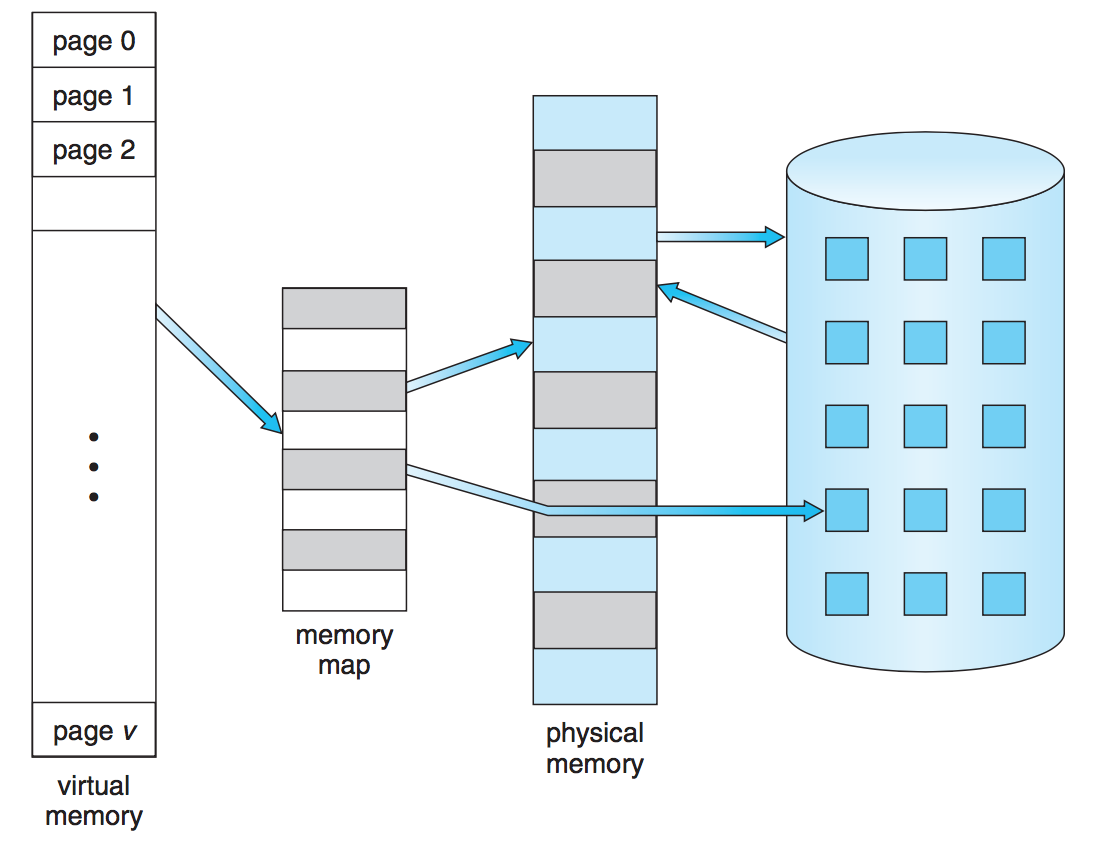
\includegraphics[width=0.85\textwidth]{images/vmem-physmem.png}
\end{center}

\end{frame}

\begin{frame}
\frametitle{Virtual Memory: Loading}

The typical approach is also like that of the cache; demand paging. 

A page is loaded into memory only if it is referenced or needed, thus preventing unnecessary disk accesses. 

\end{frame}

\begin{frame}
\frametitle{Virtual Memory: Loading}

This is also called the ``lazy'' approach.\\
\quad Though lazy is typically an insult; in this case it is not necessarily bad.  

Goal: involve disk as little as possible, because disk is extremely slow.


\end{frame}

\begin{frame}
\frametitle{Thrashing}

The fact that disk is so slow means we can get into a state called \alert{thrashing}. 

\begin{center}
	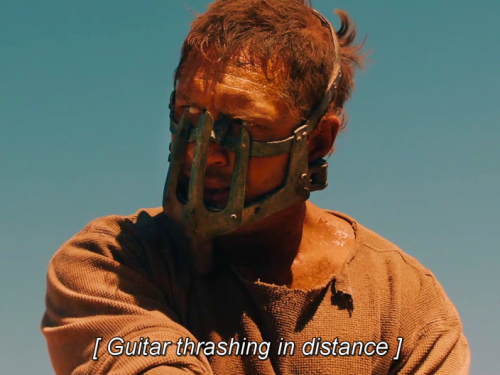
\includegraphics[width=0.4\textwidth]{images/thrashing2.png}
\end{center}

The operating system is spending most or all of its time swapping pages in and out of memory and very little actual work can get done.

We will come back to the subject of thrashing later.

\end{frame}

\begin{frame}
\frametitle{Virtual Memory: Six Steps}

\begin{enumerate}
	\item Check if the memory reference is valid or invalid.
	\item If the reference is invalid, terminate the program (segmentation fault).\\
	 If it was valid, but the page referenced is not in memory, continue.
	\item Find a free frame (or make one by evicting some other page).
	\item Request a disk read (and possibly write) to bring in the new page.
	\item When the disk read is complete, update the records.
	\item Restart the instruction that referenced the page.
\end{enumerate}


\end{frame}

\begin{frame}
\frametitle{Virtual Memory: Handling a Page Fault}

\begin{center}
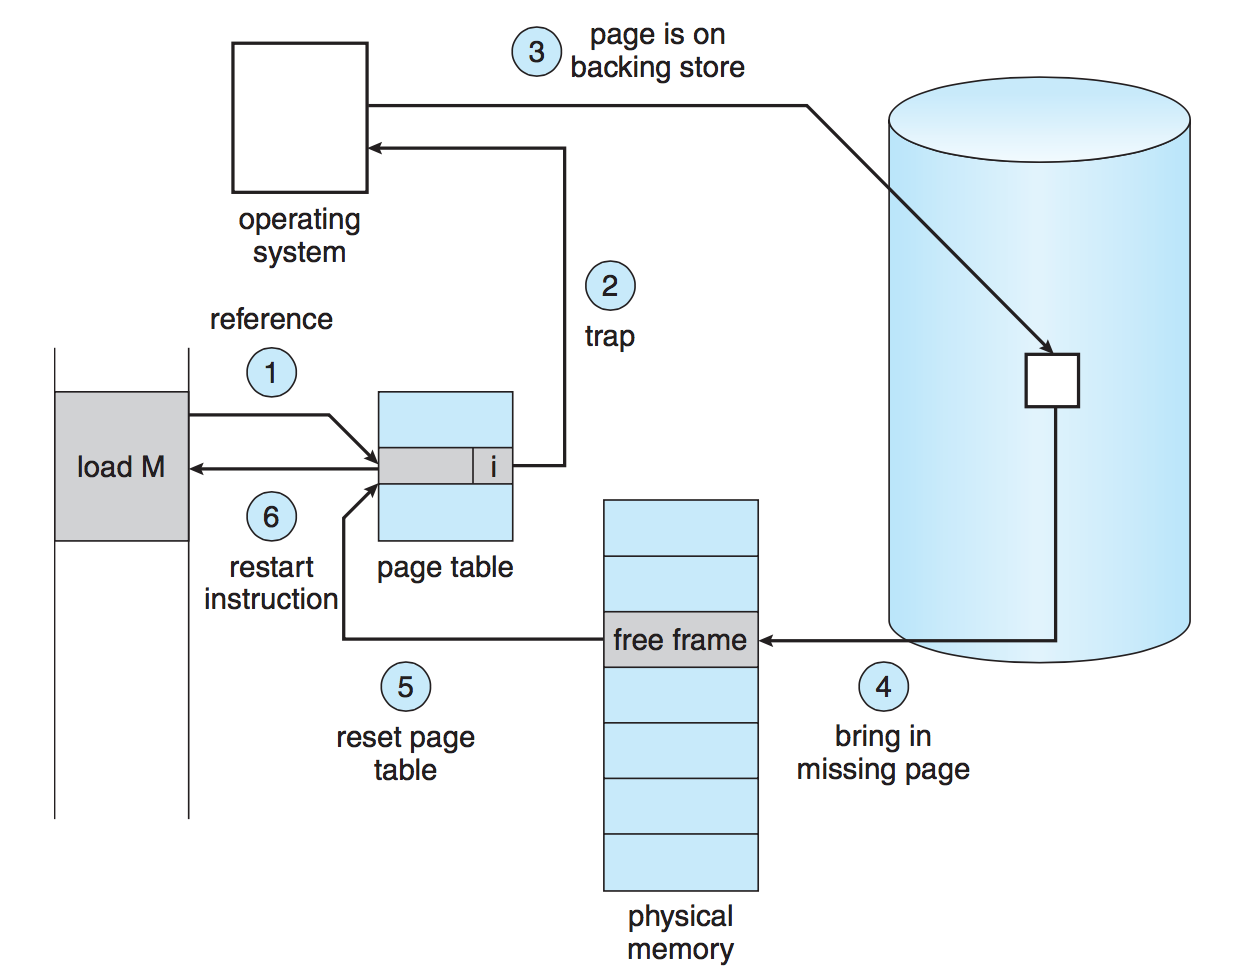
\includegraphics[width=0.9\textwidth]{images/handling-page-fault.png}
\end{center}


\end{frame}

\begin{frame}
\frametitle{Don't Waste Time}

Note that between steps 4 and 5, a significant amount of time will take place.

While the slow disk operations are going on, the process is blocked on that I/O.

In the meantime, the processor can and should be working on something else.

\end{frame}

\begin{frame}
\frametitle{Start Again (Nice Day for a..)}

The key requirement is the ability to restart any instruction after the page fault.

We save the state of the process, including all the registers and instruction pointer and so on, when the page fault occurs. 

Restart the process exactly where it was. 

After the restart, the page needed is in memory and is accessible.

\end{frame}

\begin{frame}
\frametitle{Restarting Instructions}

Page faults can occur on any memory access, even fetching the next instruction.\\
\quad If it happens at that time, the fetch operation is done again. 

If a fault happens when doing an operation that required fetching an operand, then we fetch and decode the instruction again and then fetch the operand. 

So a little bit of work may be repeated.

\end{frame}



\begin{frame}
\frametitle{Restarting an \texttt{ADD} Instruction}

Imagine an \texttt{ADD} instruction that adds \texttt{A} to \texttt{B} and stores the result in \texttt{C}. 

Fetch and decode the instruction.\\
\quad That tells us about the two operands, which must be retrieved themselves. 

Then we can add the two operands, and store the result in the target location.

\end{frame}

\begin{frame}
\frametitle{Restarting an \texttt{ADD} Instruction}

If a page fault occurs when trying to write to \texttt{C}, restart the instruction. 

Back to step one: fetch the \texttt{ADD} instruction again, then get the operands, then perform the addition, and finally write it into the destination location.

Some work is repeated here: fetching and decoding the instruction, as well as taking the operands and doing the addition. 

\end{frame}

\begin{frame}
\frametitle{Round and Round We Go}

While fetching the page containing \texttt{C} from disk, the page that contains \texttt{A} or \texttt{B} could get swapped out...

Meaning that the second run of the instruction will also produce a page fault. 

This is unlikely if using a sane replacement algorithm, because the page with \texttt{A} and \texttt{B} having just been referenced, it is a poor candidate for eviction. 

A random page replacement algorithm could result in that behaviour.

\end{frame}

\begin{frame}
\frametitle{No Do-Overs}

Can every instruction be restarted without affecting the outcome? Nope.

Example: an instruction modifies $> 1$ memory location. If we are moving a block of $n$ bytes, it is possible those bytes will straddle a page boundary.

The move operation may not be restarted if the source and destination overlap.

\end{frame}

\begin{frame}
\frametitle{No Do-Overs}

Solution: try to access the start and end addresses before the move begins. 

If one of the pages is not in memory, the page fault is triggered before any data is changed, so we can be sure the move will succeed when it actually starts. 

Another solution is temporary registers to hold overwritten location. 

If a page fault occurs, then the temporary data is restored so the instruction may be restarted without affecting the operation's correctness.

\end{frame}

\begin{frame}
\frametitle{Virtual Memory Performance}

Finding something in cache is significantly faster than main memory. 

Retrieving something from disk is dramatically slower, but computing how long it takes to retrieve a given page will follow the same principle. 

Recall from earlier the effective access time formula:

\begin{center}
	Effective Access Time = $ h \times t_{c} + (1 - h) \times t_{m}$
\end{center}


\end{frame}

\begin{frame}
\frametitle{Virtual Memory Performance}

Let's convert this to formula for virtual memory.

Replace $t_{c}$ with $t_{m}$.

Replace $t_{m}$ and $t_{d}$ (time to retrieve it from disk).

Redefine $h$ as $p$, the chance that a page is in memory:

\begin{center}
	Effective Access Time = $ p \times t_{m} + (1 - p) \times t_{d}$
\end{center}

\end{frame}



\begin{frame}
\frametitle{Virtual Memory Performance}

We can combine the caching and disk read formulae to get the true effective access time for a system where there is only one level of cache:

\begin{center}
	Effective Access Time = $ h \times t_{c} + (1 - h) ( p \times t_{m} + (1 - p) \times t_{d})$
\end{center}

This is good, but what is $t_{d}$? 

This is a measurable quantity so it is possible, of course, to just measure it.

We expect $p$ to be large if our paging algorithm is any good.

\end{frame}



\begin{frame}
\frametitle{Handling a Page Fault}

Handling a page fault is a ``simple'' 16 step process!

... You can see why it is something we wish to avoid.

\begin{enumerate}
	\item Trap to the operating system.
	\item Save the user registers and process state.
	\item Identify this interrupt as a page fault.
	\item Check that the page reference was legal. 
	\begin{enumerate}
		\item If so, determine the location of the page on disk.
		\item If not, terminate the requesting program. Steps end here.
	\end{enumerate}
	\setcounter{pf}{\theenumi}
\end{enumerate}

\end{frame}

\begin{frame}
\frametitle{Handling a Page Fault}
\begin{enumerate}
	\setcounter{enumi}{4}
	\item Figure out where to place the page in memory (use our replacement algorithm).
	\item Is the frame we have selected currently filled with a page that has been modified? 
	\begin{enumerate}
		\item If so, schedule a disk write to flush that page out to disk. The disk write request is placed in a queue.
		\item If not, go to step 11.
	\end{enumerate} 
	\item Wait for the disk write to be executed. The CPU can do something else in the meantime, of course.
	\item Receive an interrupt when the disk write has completed.
\end{enumerate}

\end{frame}

\begin{frame}
\frametitle{Handling a Page Fault}

\begin{enumerate}
	\setcounter{enumi}{8}
	\item Save the registers and state of the other process if the CPU did something else.
	\item Update the page tables to reflect the flush of the replaced page to disk. Mark the destination frame as free.
	\item Issue a disk read request to transfer the page to the free frame.
	\item As before, while waiting, let the CPU do something else.
	\item Receive an interrupt when the disk has completed the I/O request.
	\item Save the registers and state of the other process (if necessary).
	\item Update the page tables to reflect the newly read page.
	\item Restore the state of and resume execution of the process that encountered the page fault, restarting the instruction that was interrupted.
\end{enumerate}


\end{frame}

\begin{frame}
\frametitle{Page Faults are Slow}

The slow step in all this the amount of time it takes to load the page from disk. 

Restarting the process and managing memory and such take 1 to 100~$\mu$s.

If a HDD has latency of 3~ms, seek time is 5~ms, and transfer time 0.05~ms. 

So the latency plus seek time is the limiting component, and it's several orders of magnitude larger than any of the other costs in the system. 

This is for servicing a request; don't forget that several requests may be queued, making the time even longer.

\end{frame}

\begin{frame}
\frametitle{Page Faults are Slow}

Thus the disk read term $t_{d}$ dominates the effective access time equation. 

If memory access takes 200~ns and a disk read 8~ms, we can roughly estimate the access time in nanoseconds as $(1-p) \times 8~000~000$. 

If the page fault rate is high, performance is awful. 

If performance of the computer is to be reasonable, say around 10\%, the page fault rate has to be very, very low. On the order of $10^{-6}$. 

\end{frame}

\begin{frame}
\frametitle{SSDs: The Way of the Future}

And now you also know why solid state drives, SSDs, are such a huge performance increase for your computer. 

Instead of spending time measured in the milliseconds to find a page on disk, SSDs produce the data with times that look more like memory reads.

(Take the technical elective Programming for Performance to learn why this, while faster, is not fast enough.)


\end{frame}

\begin{frame}
\frametitle{Swap File}

We have not yet covered file systems, but files tend to come with a bunch of overhead for file creation and management. 

To avoid this, the system usually has a ``swap file'' which is just one giant file or partition of the hard drive. 

The system can get better performance by just dealing with the swap file as one big file (block) and not tiny individual files.

\end{frame}

\begin{frame}
\frametitle{Thrashing}
This topic was previously introduced, and now we'll come back to it.

The quick definition of thrashing still applies.

Aside from intentionally depriving the system of RAM, how can we get into this state, and how can we get out of it?


\end{frame}

\begin{frame}
\frametitle{Thrashing}

In simple operating systems, the logic that controlled how many processes to run at a time would rely just on the CPU utilization. 

If CPU utilization is low, the CPU needs more work to do! 

\begin{center}
	
\includegraphics[width=0.4\textwidth]{images/backtowork.jpg}
\end{center}

\end{frame}

\begin{frame}
\frametitle{Thrashing}

Assign it more work by starting or bringing more processes into memory. 

The global page replacement policy is used here, so when a process gets a page fault, it takes a frame from another process. 

Under most circumstances, this works just fine.

\end{frame}

\begin{frame}
\frametitle{Downward Spiral}

This situation can run until one process starts to have a lot of page faults. 

This is not unreasonable; a compiler might be finished with reading and parsing the input files and moving to generation of binary code. 

This requires a whole bunch of new instructions pages, plus pages for output. 

When this process does so, it starts taking pages from other processes.

\end{frame}

\begin{frame}
\frametitle{Downward Spiral}

The victim processes need the pages they had, so when they get a turn to run, they too start generating page faults. 

So more and more requests are queued up for memory writes and reads, so the CPU is not very busy. 

Here's the fatal mistake: seeing that the CPU is not very busy, the OS schedules \textbf{more} programs to run.  

\end{frame}

\begin{frame}
\frametitle{The Doom in Thrashing}

A new process getting started will need at least the minimum number of pages. 

These have to come from somewhere, so they will necessarily come from the pages currently belonging to other processes. 

This causes more page faults, more time spent paging, lower CPU utilization...\\
\quad Prompting the OS to start more processes. 
\end{frame}

\begin{frame}
\frametitle{Whiplash!}

No more work is getting done, because the system spends all its time moving pages into and out of memory, thrashing all around, acting like a maniac.

\begin{center}
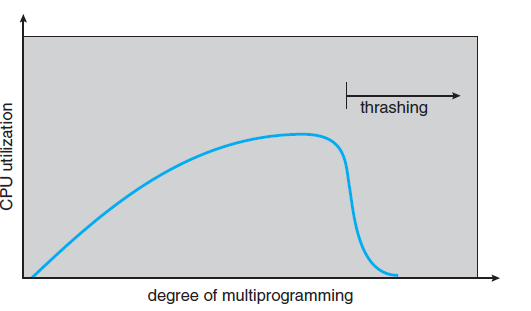
\includegraphics[width=0.75\textwidth]{images/thrashing.png}
\end{center}

\end{frame}

\begin{frame}
\frametitle{Breaking the Spiral}

To increase CPU utilization we need to stop the thrashing...\\
\quad which means we need \textbf{fewer} programs in memory at a time. 

CPU usage alone is not a sufficient indicator of whether more or fewer processes need to be running right now. 

It also matters \textit{why} the CPU utilization is low. Another reason that might cause low CPU usage is, as you may recall, deadlock. 


\end{frame}

\begin{frame}
\frametitle{Check Assumptions}

We've assumed so far that temporal and spatial locality are real.

Are they? 

How would we know?

\end{frame}

\begin{frame}
\frametitle{Check Assumptions}

\begin{center}
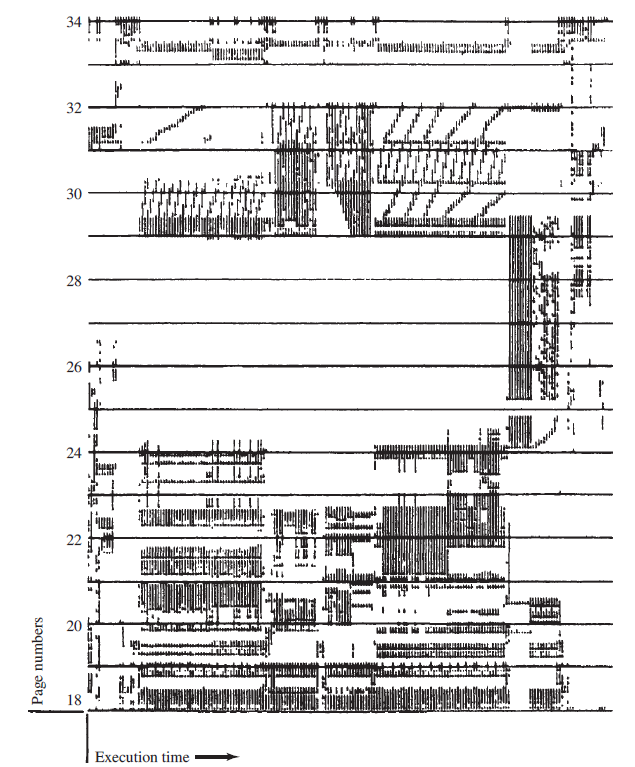
\includegraphics[width=0.55\textwidth]{images/locality.png}
\end{center}


\end{frame}




\end{document}

